\documentclass[12pt, a4paper, brazilian]{article}
\usepackage{fix-cm}

\usepackage[a4paper,
            top=3cm, bottom=2cm,
            left=3cm, right=2cm]{geometry}

\usepackage[num, overcite]{abntex2cite}
\citebrackets[]
\makeatletter
\renewcommand\@biblabel[1]{[#1] }
\makeatother

\usepackage{subcaption}
\usepackage{booktabs}
\usepackage{amsmath, amsfonts, amsthm, bm}
\usepackage{newtxtext, newtxmath, mathtools}
\usepackage[brazilian]{babel}
\usepackage[T1]{fontenc}
\usepackage{indentfirst}
\usepackage{microtype}
\usepackage{fancyhdr}
\usepackage{graphicx}
\usepackage{ragged2e}
\usepackage{multirow}
\usepackage{multicol}
\usepackage{setspace}
\usepackage{icomma}
\usepackage{array}
\usepackage{float}
\usepackage{tikz}

\usepackage{silence}
\WarningFilter{latex}{Command \showhyphens has changed}

\onehalfspacing
\setlength{\parindent}{1.25cm}
\setlength{\parskip}{0.4\baselineskip}
\justifying

\usepackage{titlesec}

\newcommand{\titlefix}{
  \hyphenpenalty=10000
  \exhyphenpenalty=10000
  \emergencystretch=2em
}

\captionsetup{
    justification=centering
}

\titleformat{\section}
{\normalsize\bfseries\titlefix}
{\thesection.}
{0.5em}
{}

\titlespacing*{\section}
{0.75cm}
{1.5\baselineskip}
{0.8\baselineskip}

\titleformat{\subsection}
{\normalsize\bfseries\titlefix}
{\thesubsection.}
{0.5em}
{}

\titlespacing*{\subsection}
{1.5cm}
{1.2\baselineskip}
{0.6\baselineskip}

\titleformat{\subsubsection}
{\normalsize\bfseries\titlefix}
{\thesubsubsection.}
{0.5em}
{}

\titlespacing*{\subsubsection}
{2.25cm}
{1.0\baselineskip}
{0.4\baselineskip}

\titleformat{name=\section,numberless}
{\normalsize\bfseries\centering\titlefix}
{}
{0em}
{}

\titlespacing*{name=\section,numberless}
{0cm}
{1.5\baselineskip}
{0.8\baselineskip}

\newcounter{rownum}
\setcounter{rownum}{0}

\newcolumntype{N}{>{\stepcounter{rownum}\therownum.}l}

\begin{document}
\newpage

\pagestyle{empty}

\begin{center}

\noindent
\begin{minipage}[c]{0.65\textwidth}
{\Large\bfseries
Determinação da gravidade por meio do pêndulo simples
}
\vspace{0.35cm}

{\normalsize
\textbf{
Caio Schaden Ishida\textsuperscript{1},
Felipe Osternes da Silva\textsuperscript{1},
João Victor Evers Cordeiro\textsuperscript{1},
Paulo Vinícius Rodrigues de Azevedo\textsuperscript{1},
Rafael Sakata Suzuki\textsuperscript{1}}
}

\vspace{0.15cm}

{\footnotesize
\textsuperscript{1}\textit{Instituto Tecnológico de Aeronáutica -- ITA,
Praça Marechal Eduardo Gomes, 50 -- Vila das Acácias,
São José dos Campos -- SP, Brasil.
}
}   
\end{minipage}
\hfill
\begin{minipage}[t]{0.25\textwidth}
    \vspace{-2.7cm}
    \centering
    
\includegraphics[width=1\linewidth]{ita_rgb.jpg}
\end{minipage}

\vspace{0.20cm}

\end{center}

\begin{center}
{\normalsize\bfseries Resumo}
\end{center}

{\footnotesize
\setlength{\parindent}{0pt}
\setlength{\parskip}{0pt}
Neste trabalho, foi realizada a determinação experimental da aceleração da gravidade $g$ a partir da medição do período de um pêndulo simples. Além da obtenção do valor de $g$, o experimento teve como objetivo comparar quatro metodologias distintas para a determinação do período de oscilação, que incluem dois métodos baseados no uso de cronômetros manuais, a análise de uma gravação em vídeo por meio de software e a medição automática utilizando uma fotoporta. A comparação entre os métodos permite avaliar suas respectivas precisões e limitações, bem como verificar a influência da técnica de medição sobre o valor experimental obtido para a aceleração da gravidade.
}

\vspace{0.2cm}

{\footnotesize
\setlength{\parindent}{0pt}
\setlength{\parskip}{0pt}
\textbf{Palavras-chave:}
Pêndulo simples, aceleração da gravidade, métodos de medição.
}

\vspace{0.5cm}
\pagestyle{fancy}
\fancyhf{}
\fancyfoot[R]{\thepage}
\renewcommand{\headrulewidth}{0pt}
\setcounter{page}{1}

\begin{multicols}{2}
    \section{Introdução}
	Um pêndulo simples é uma montagem experimental caracterizada por meio da suspensão utilizando um fio, suposto ideal, de uma massa qualquer $m$ em um ponto em torno do qual ela possa oscilar livremente. Se consideradas pequenas amplitudes angulares, o movimento oscilatório pode ser aproximado para um movimento harmônico simples de período $T$, o qual depende da gravidade $g$ e da distância fixa $l$ entre o centro de massa do objeto suspenso e o ponto de suspensão.

	Considere uma massa esférica $m$ presa, por meio de um fio ideal, a um ponto fixo no teto em um meio onde pode ser desprezada a resistência do ar, assim como mostra a Figura \ref{fig:pendulo_intro}.

	\begin{figure}[H]
		\centering
		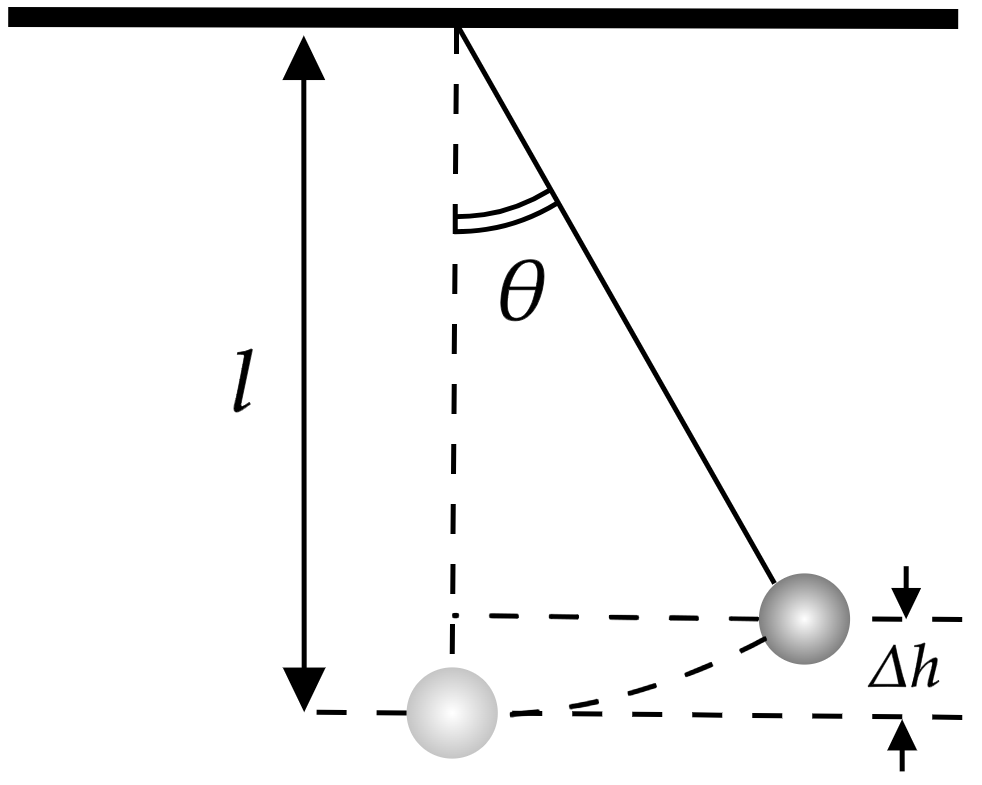
\includegraphics[width = 0.95\linewidth]{pendulo_intro.png}

		\caption{Esquematização de um pêndulo simples}
		\label{fig:pendulo_intro}
	\end{figure}

	A distância fixa entre o ponto de apoio no teto e o centro de massa da esfera é $l$ e a suposição de idealidade do fio inclui inextensibilidade e massa aproximadamente nula. Adotando um sistema de coordenadas polares com pivô no ponto de apoio, a Equação \ref{eq:vel} é a velocidade da massa esférica, que não possui componentes radiais.

	\begin{equation}\label{eq:vel}
		v = l\dot\theta
	\end{equation}

	em que $\dot\theta$ é a primeira derivada temporal de $\theta(t)$, o ângulo que o fio do pêndulo faz com a vertical em um tempo $t$. Também, para um dado $\theta$, a variação de altura $\Delta h(\theta)$ em relação de equilíbrio é dada pela Equação \ref{eq:deltah}, segundo sugere a geometria da Figura \ref{fig:pendulo_intro}.

	\begin{equation}\label{eq:deltah}
		\Delta h = l(1-\cos\theta)
	\end{equation}

	Por meio disso, é possível escrever a energia total da partícula, que terá uma compente cinética e outra potencial gravitacional, assim como faz a Equação \ref{eq:energianaprox}.

	\begin{equation}\label{eq:energianaprox}
		E_{mec} = \frac{1}{2}ml^2\dot\theta^2 + mgl(1-\cos\theta)
	\end{equation}

	que descreve uma oscilação genérica em que o período depende da amplitude angular. Pode-se considerar, portanto, pequenas amplitudes angulares, de forma que $|\theta(t)|\le\theta_0\ll 1\ \text{rad}$. Nesse regime, pode-se considerar a Série de Maclaurin para $\cos\theta$, expressa na Equação \ref{eq:mclaurincos}.

	\begin{equation}\label{eq:mclaurincos}
		\cos\theta = 1 - \frac{1}{2}\theta^2 + \mathcal{O}(\theta^4)
	\end{equation}

	cuja aproximação em segunda ordem resulta em um erro relativo menor que $0,07\%$ para $\theta\le 20^\circ\approx 0,35\ \text{rad}$. Portanto, usando a Série de Maclaurin truncada até segunda ordem, obtém-se uma expressão para a energia total dada segundo a Equação \ref{eq:energia}.

	\begin{equation}\label{eq:energia}
		E_{mec}\approx \frac{1}{2}ml^2\dot\theta^2+\frac{1}{2}mgl\theta^2
	\end{equation}

	que é idêntica à energia do movimento harmônico simples de frequência angular $\omega$ para uma variável $x$, expressa na Equação \ref{eq:energiaMHS}.

	\begin{equation}\label{eq:energiaMHS}
		E_{MHS} = \frac{1}{2}m\dot x^2 + \frac{1}{2}m\omega^2x^2
	\end{equation}

	Portanto, comparando as Equações \ref{eq:energia} e \ref{eq:energiaMHS}, pode-se obter a frequência angular $\omega = 2\pi/T$ do Movimento Harmônico que o pêndulo executa em pequenas amplitudes, assim como está na Equação \ref{eq:omega}.\cite{springer}

	\begin{equation}\label{eq:omega}
		\omega^2=\frac{g}{l}
	\end{equation}

	de onde, obtém-se a Equação \ref{eq:periodo}, que expressa o período de oscilação do pêndulo em termos da aceleração da gravidade $g$ e da distância fixa entre o ponto de apoio e o centro de massa da esfera $l$.

	\begin{equation}\label{eq:periodo}
		T=2\pi\sqrt{\frac{l}{g}}
	\end{equation}

	Neste experimento, buscou-se determinar o valor da aceleração da gravidade $g$ por meio da medição do período de um pêndulo simples. Também, buscou-se obter o período do pêndulo por meio de quatro métodos diferentes, cronômetro de mão, usando cronômetro de bancada, fotoporta e uma gravação de 240 fps, comparando-se os resultados obtidos para os períodos e para a aceleração da gravidade por meio de testes de hipótese.

	\section{Procedimento experimental}
	Foram conduzidos quatro métodos experimentais diferentes para medição do período do pêndulo simples, todos eles utilizando o arranjo experimental representado na Figura \ref{fig:pendulo}, em que uma massa esférica de metal é presa em um suporte universal por meio de um fio de \textit{nylon} suposto aproximadamente ideal. A distância entre o ponto de apoio no suporte e o centro de massa da esfera $l=(35,00\pm 0,05)\ \text{cm}$ foi medida com um trena e permanenceu constante em todos os experimentos.

	\begin{figure}[H]
		\centering
		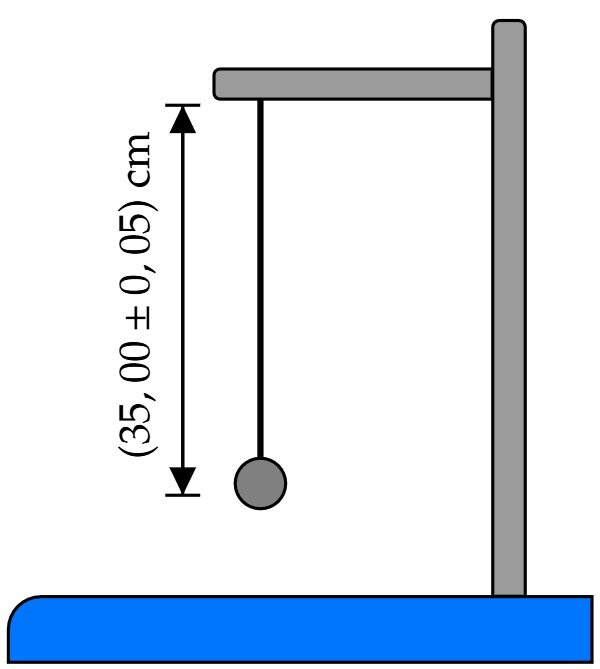
\includegraphics[width=0.75\linewidth]{pendulo.jpeg}
		\caption{Arranjo experimental utilizado para a determinação da gravidade}
		\label{fig:pendulo}
	\end{figure}

	Nos dois primeiros métodos utilizados, foi o medido o tempo de dez oscilações do pêndulo simples, visando minimizar as incertezas relativas causadas pelo tempo de reação e outros erros aleatórios. O procedimento foi repetido cem vezes e cada tempo foi medido, simultaneamente, com um cronômetro de mão da marca CASIO e um cronômetro de bancada da marca Cidepe, como mostra a Figura \ref{fig:cronom}. Totalizaram-se, portanto, 200 medidas por meio destes dois métodos.

	\begin{figure}[H]
		\centering

		\begin{subfigure}[b]{0.66\linewidth}
			\centering
			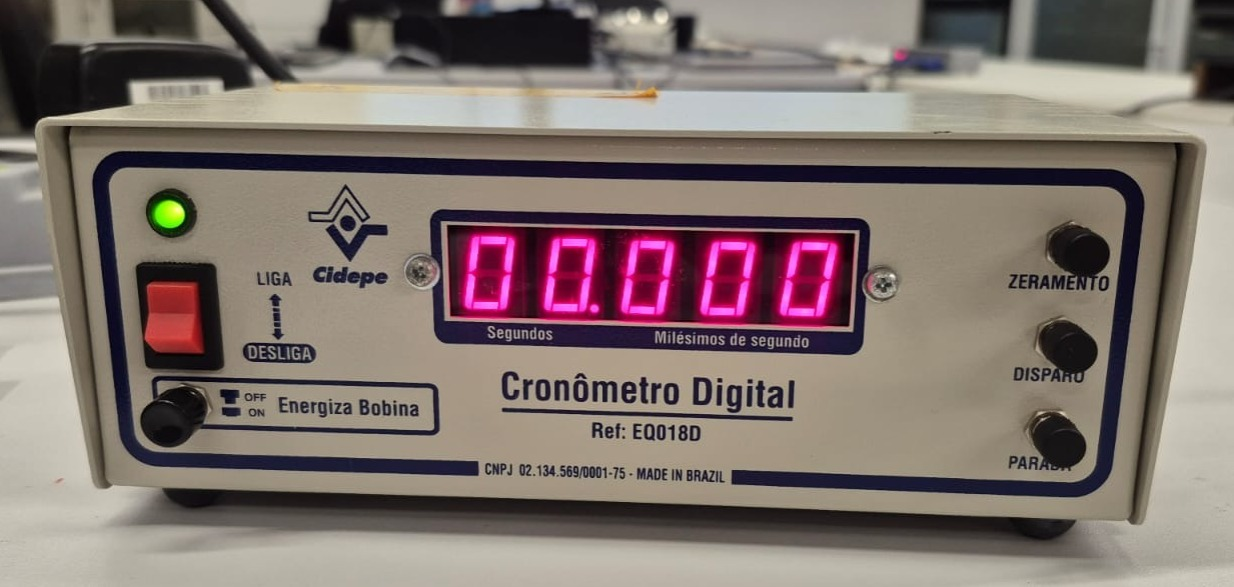
\includegraphics[width=\linewidth]{cronom_mesa.jpeg}
			\caption{Cronômetro\\ de mesa}
			\label{fig:sub_a}
		\end{subfigure}
		\hfill
		\begin{subfigure}[b]{0.30\linewidth}
			\centering
			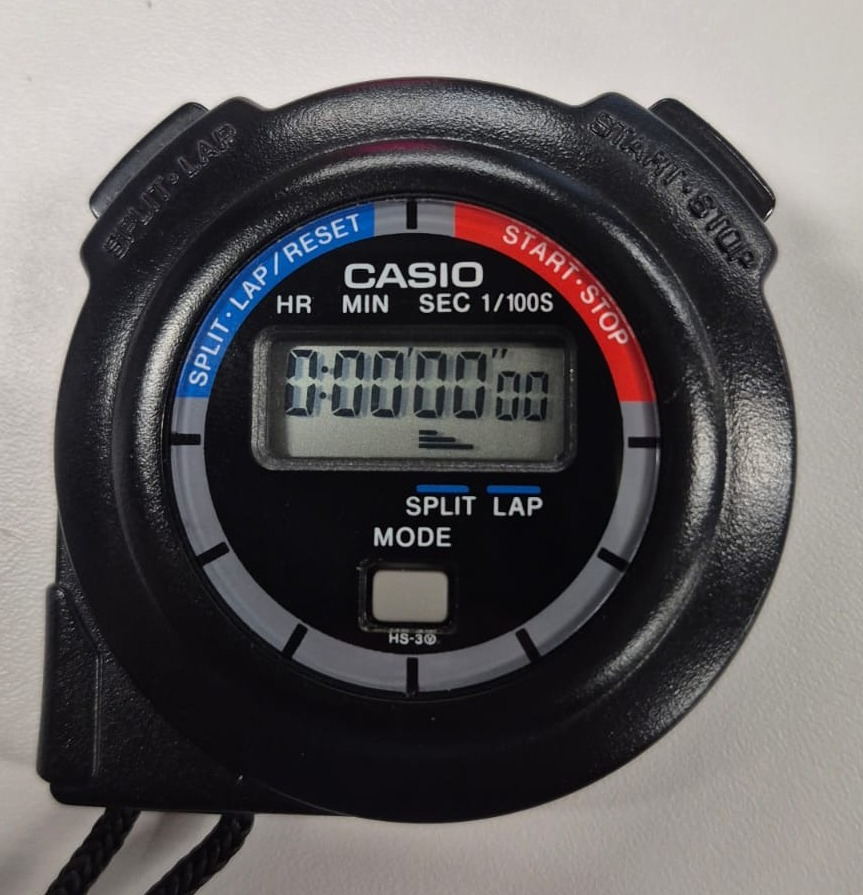
\includegraphics[width=\linewidth]{cronom_mao.jpeg}
			\caption{Cronômetro de mão}
			\label{fig:sub_b}
		\end{subfigure}

		\caption{Instrumentos de medição utilizados}
		\label{fig:cronom}
	\end{figure}

	Também, utilizou-se o aplicativo \textit{Tracker} para a análise da gravação em 240 fps de um período do pêndulo simples, obtida por meio de um celular \textit{Samsung Galaxy S24FE}. No aplicativo, determinou-se a diferença em quadros entre duas passagens consecutivas na posição de máximo. A partir disso, determina-se o tempo de um período sabendo-se que um quadro corresponde a $1/240\ \text{s}$. Como incerteza instrumental associada a essa medida, utilizou-se o tempo de um quadro, ou seja, $\Delta t=1/240\ \text{s}\approx 0,004\ \text{s}$.

	Por fim, utilizou-se uma fotoporta da marca PASCO acoplada na montagem experimental da Figura \ref{fig:pendulo} para a medição do período do pêndulo por meio de uma interface \textit{ScienceWorkshop 750} que se comunica com o \textit{software} PASCO correspondente. A Figura \ref{fig:fotoporta} exibe a montagem experimental adaptada.

	\begin{figure}[H]
		\centering

		\begin{subfigure}[b]{0.60\linewidth}
			\centering
			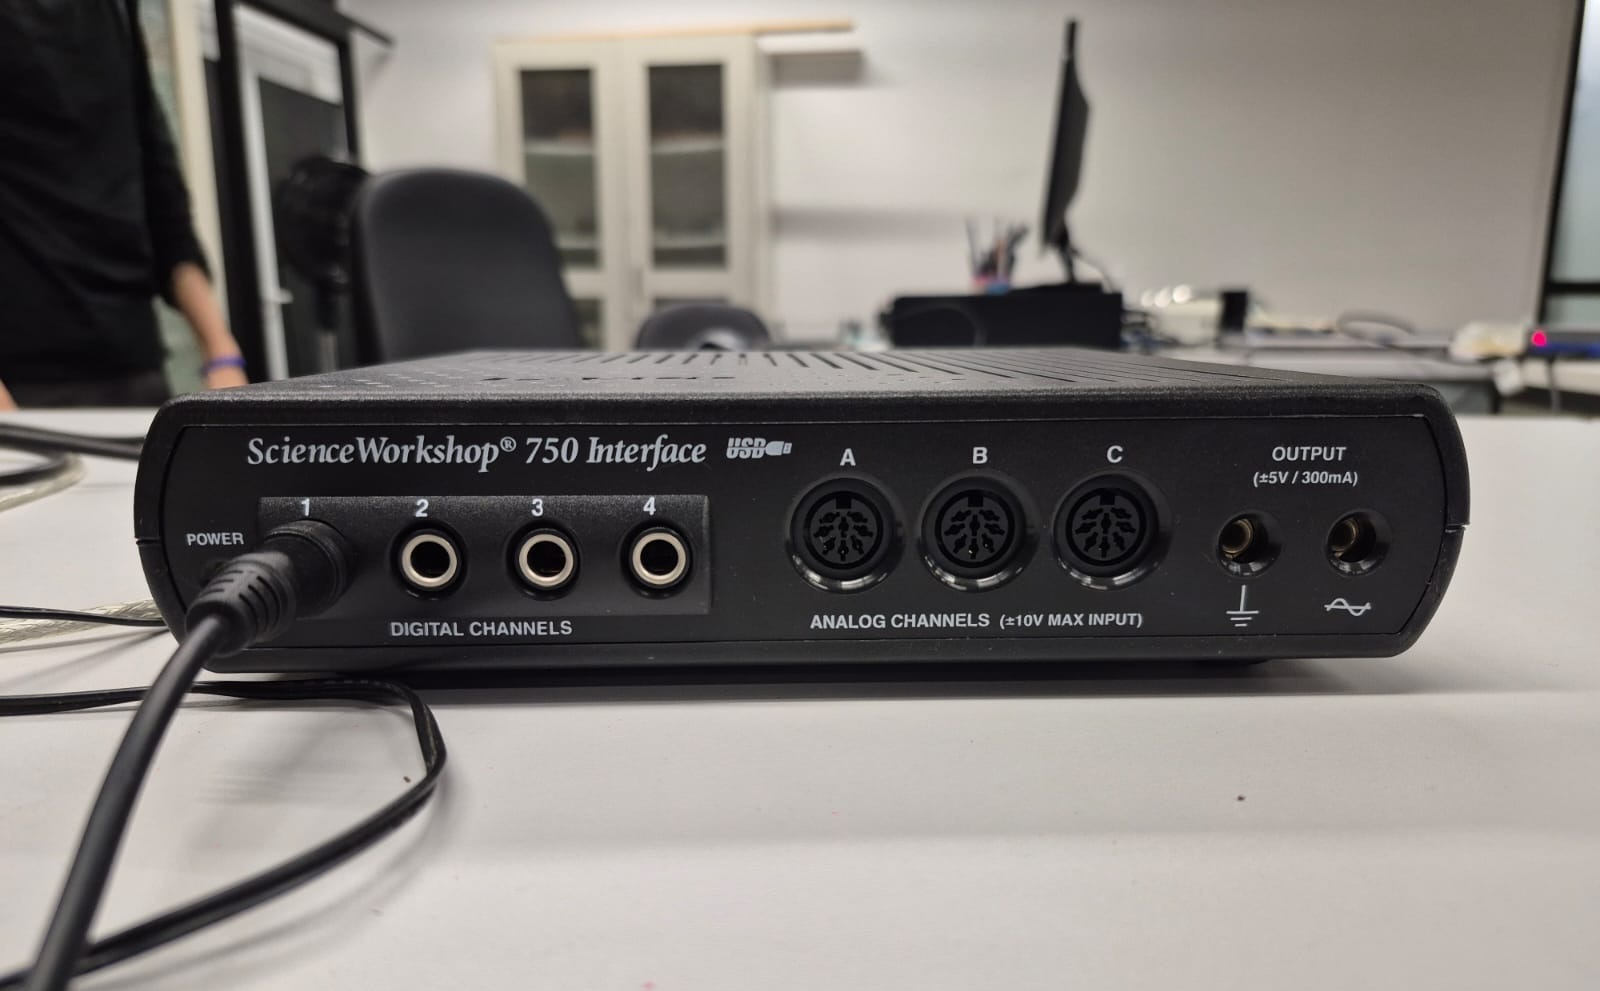
\includegraphics[width=\linewidth]{interface.jpeg}
			\caption{Interface de comunicação}
			\label{fig:sub_a_int}
		\end{subfigure}
		\hfill
		\begin{subfigure}[b]{0.38\linewidth}
			\centering
			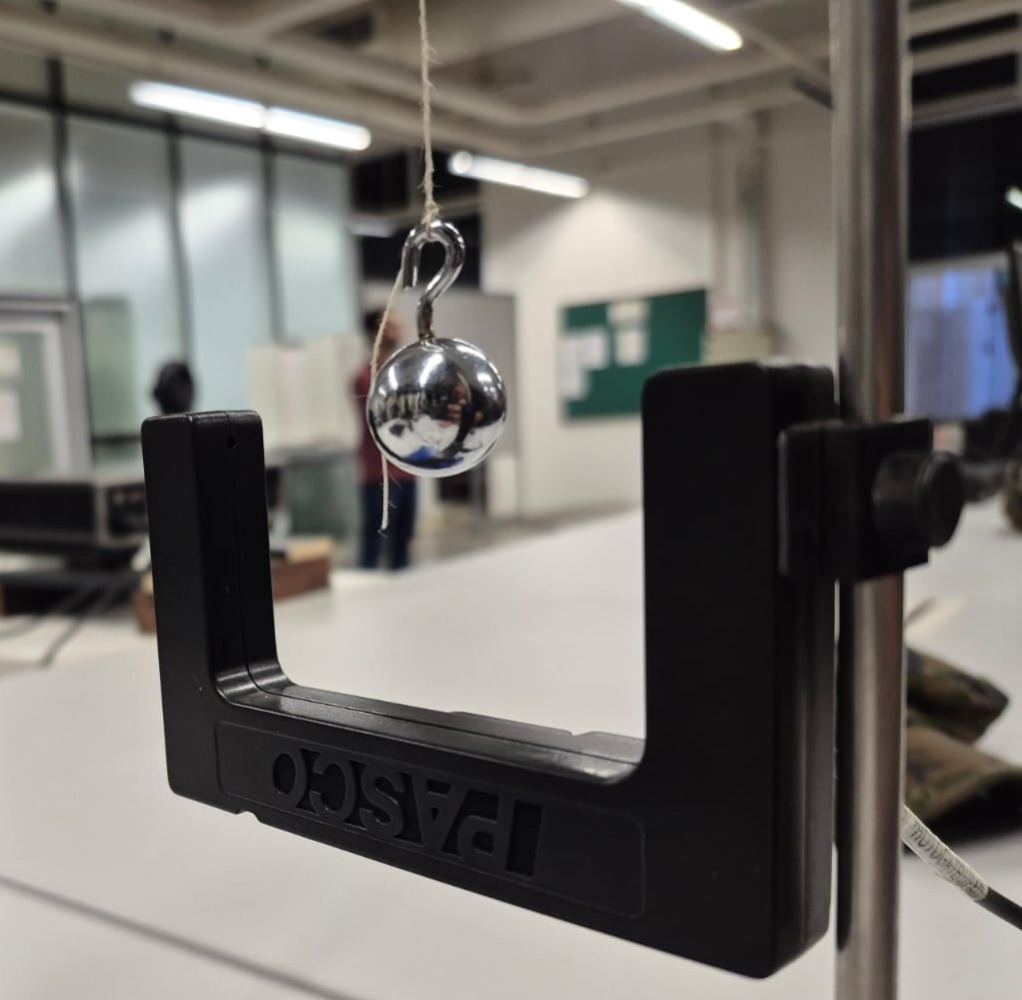
\includegraphics[width=\linewidth]{fotoporta.jpeg}
			\caption{Fotoporta}
			\label{fig:sub_b_int}
		\end{subfigure}

		\caption{Instrumentos de medição utilizados}
		\label{fig:fotoporta}
	\end{figure}

	A fotoporta identifica cada passagem do pêndulo pela posição vertical e calcula o período por meio de uma lógica interna que contabiliza a extensão não nula da esfera. Para esse método, repetiu-se 100 vezes a medição do período do pêndulo, com uma incerteza correspondente a menor divisão de medição igual a $0,0001\ \text{s}$.

	\section{Resultados e Discussão}

	Com base nas metodologias apresentadas na seção anterior, foram conduzidos quatro experimentos para a determinação do período do pêndulo. A Tabela \ref{tab:resultados}
	contém os valores e incertezas finais dos períodos medidos utilizando cronômetro de mão ($T^{(1)}$), cronômetro de bancada ($T^{(2)}$), fotodiodo ($T^{(3)}$) e \textit{tracker} ($T^{(4)}$), as estimativas obtidas da aceleração da gravidade local ($g^{(1)}$ até $g^{(4)}$, respectivamente), e o valor de referência da aceleração local da gravidade $g_{0}$.

	\begin{table}[H]
		\centering
		\caption{Medidas de período e aceleração local da gravidade, incluindo o valor de referência $g_{0}$}
		\begin{tabular}{l l l}
			\hline
			Grandeza                      & Valor   & Incerteza \\[0.5ex]
			\hline
			$T^{(1)}\ \mathrm{(s)}$       & $1,174$   & 0,012     \\
			$T^{(2)}\ \mathrm{(s)}$       & $1,172$   & 0,012     \\
            $T^{(3)} \mathrm{(s)}$        & $1,19082$ & $0,00013$ \\
			$T^{(4)} \mathrm{(s)}$        & $1,196$   & $0,012$   \\
			$g^{(1)}\ \mathrm{(m/s^{2})}$ & $10,03$   & 0,15      \\
			$g^{(2)}\ \mathrm{(m/s^{2})}$ & $10,06$   & 0,15      \\
			$g^{(3)} \mathrm{(m/s^{2})}$  & $9,744$   & $0,028$   \\
			$g^{(4)} \mathrm{(m/s^2)} $   & $9,66$    & $0,19$    \\
            $g_{0}\ \mathrm{(m/s^{2})}$   & $9,786$   &           \\
			\hline
		\end{tabular}
		\label{tab:resultados}
	\end{table}

	A fim de visualizar os dados obtidos, a Figura \ref{fig:histograma} contém os histogramas dos valores de período medidos comparados a distribuições gaussianas de mesma média e desvio padrão.

	\begin{figure}[H]
		\centering
		\caption{Histograma de frequência das medidas}
        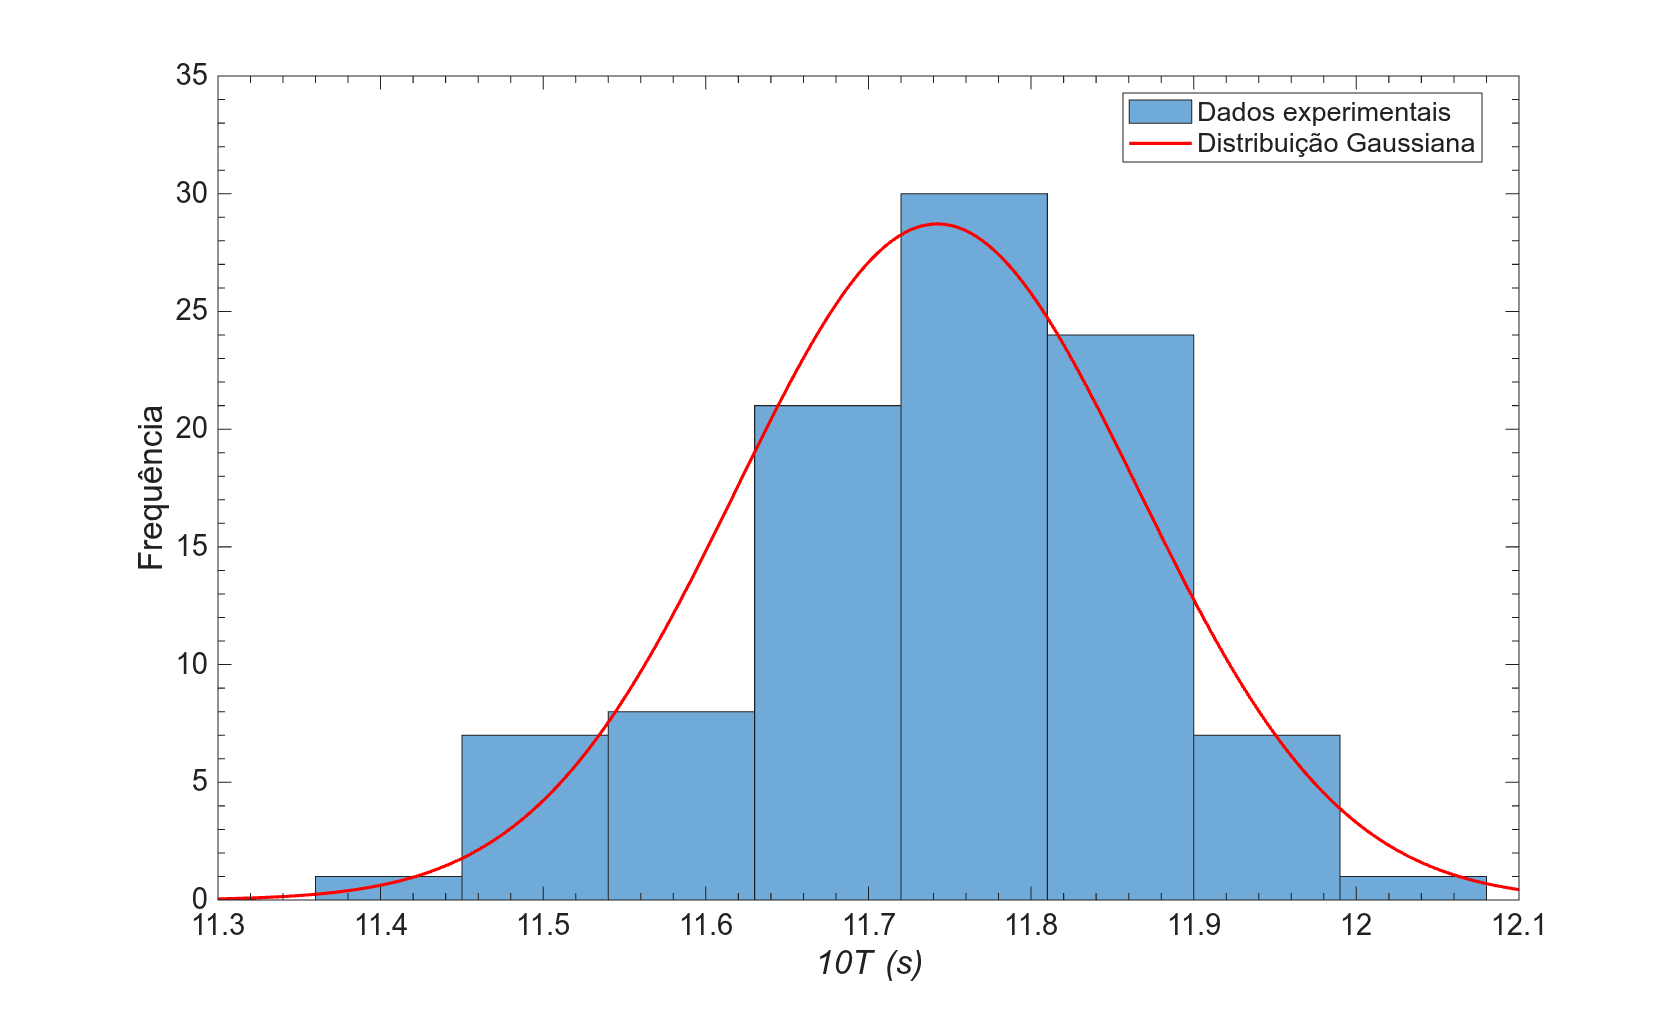
\includegraphics[width=\linewidth]{figura_cm.png}
        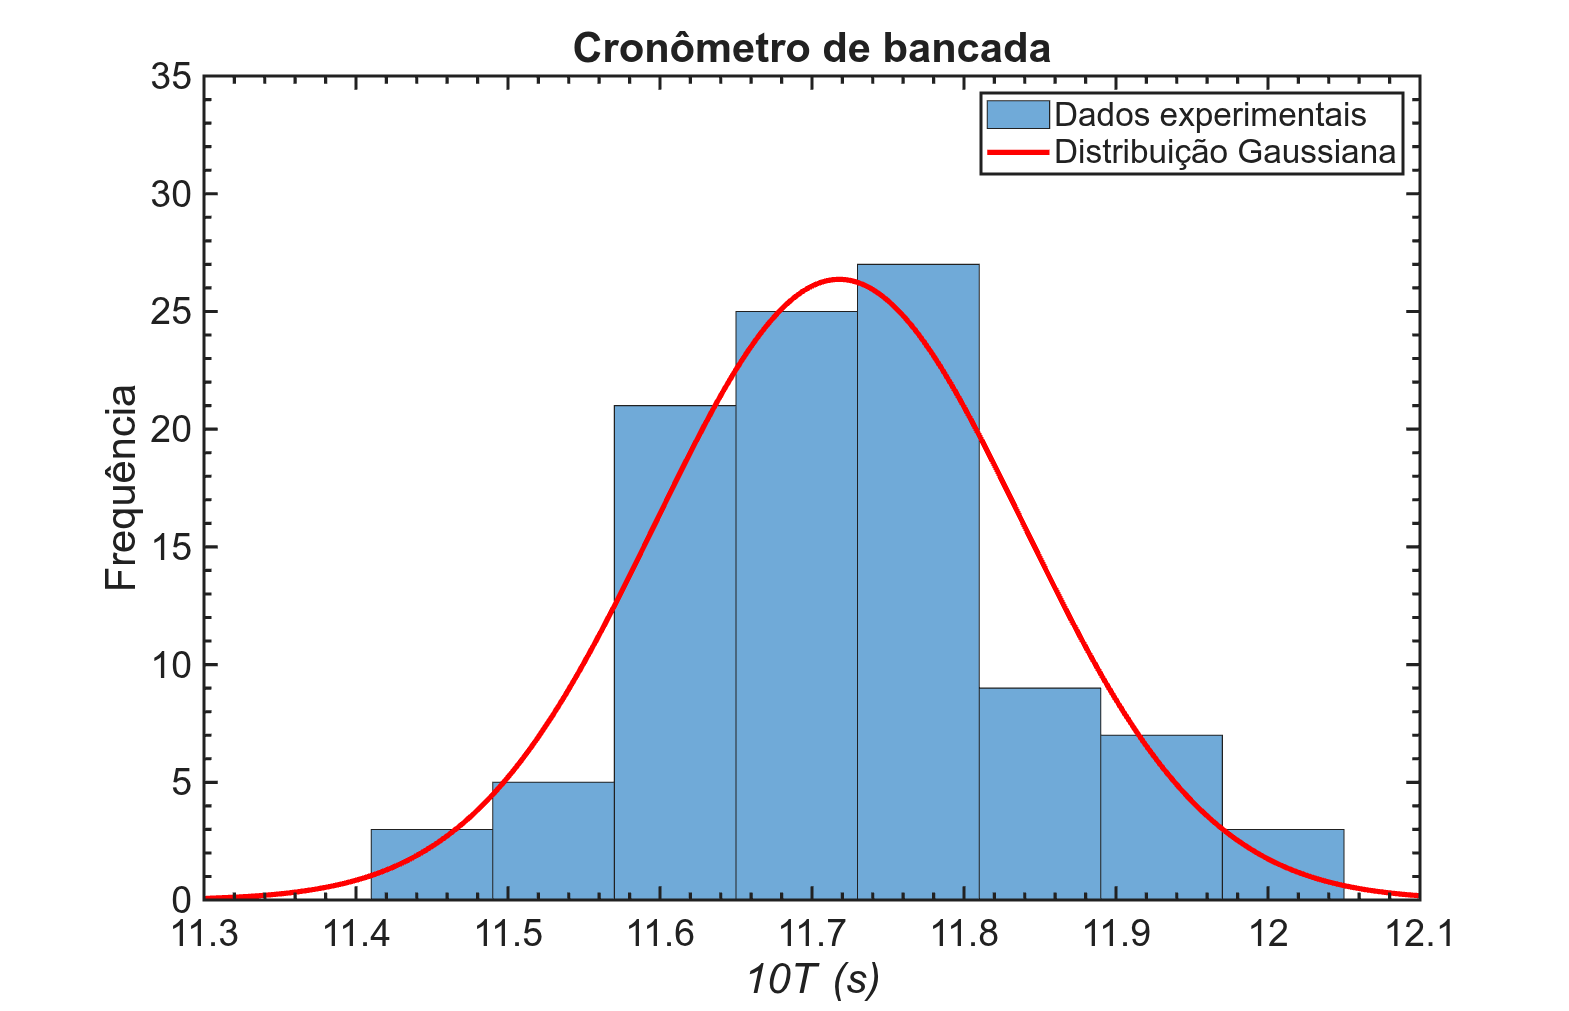
\includegraphics[width=\linewidth]{figura_cb.png}
        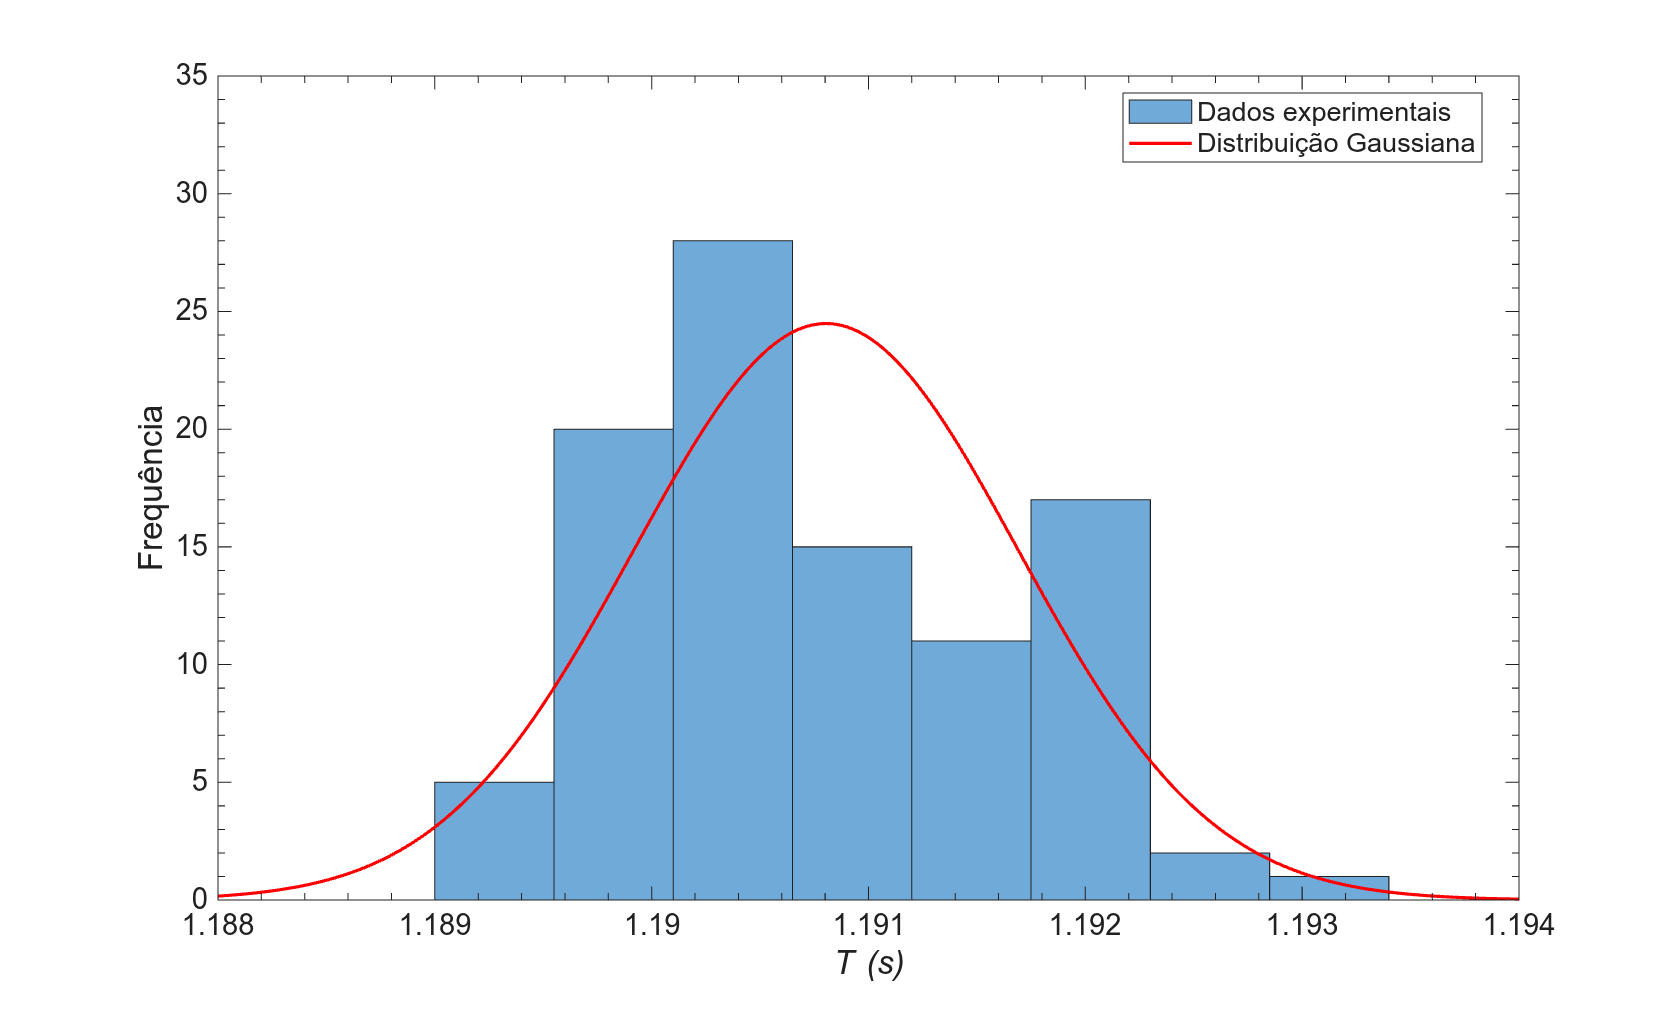
\includegraphics[width=\linewidth]{figura_fd.png}
		\label{fig:histograma}
	\end{figure}
    Com esses dados, pode-se estudar a qualidade do ajuste gaussiano utilizando o coeficiente de aderência $q$, descrito pela Equação \ref{eq:comp}:
	\begin{equation}\label{eq:comp}
		q = \frac{\sum_{i}(f_{Gauss,i}-{f_{hist}})^2}{\sum_{i}(f_{hist, i}-\overline{f_{hist}})^2}
	\end{equation}

	Nesse cálculo, o coeficiente $q$ assume valor nulo se a distribuição ajusta perfeitamente os dados experimentais obtidos, enquanto seu valor se distancia de $0$ quando a distribuição proposta não ajusta bem os dados. A Tabela \ref{tab:determ} contém os valores de $q$ para cada cada experimento:
   	\begin{table}[H]
	\centering
	\caption{Coeficientes de aderência para os experimentos 1, 2 e 3}
	\begin{tabular}{l l}
		\hline
		Experimento               & $q$ \\[0.5ex]
		\hline
		Cronômetro de mão (1)     & 0.095 \\
        Cronômetro de bancada (2) & 0.089 \\
        Fotodiodo (3)             & 0.469 \\
		\hline
	\end{tabular}
	\label{tab:determ}
\end{table}

	Visualmente, a Figura \ref{fig:desvios} é uma representação gráfica para os desvios da distribuição Gaussiana em relação às observações experimentais para cada uma dos métodos para medição do período, dados por $\delta = f_{Gauss} - f_{hist}$.

    \begin{figure}[H]
	\centering
	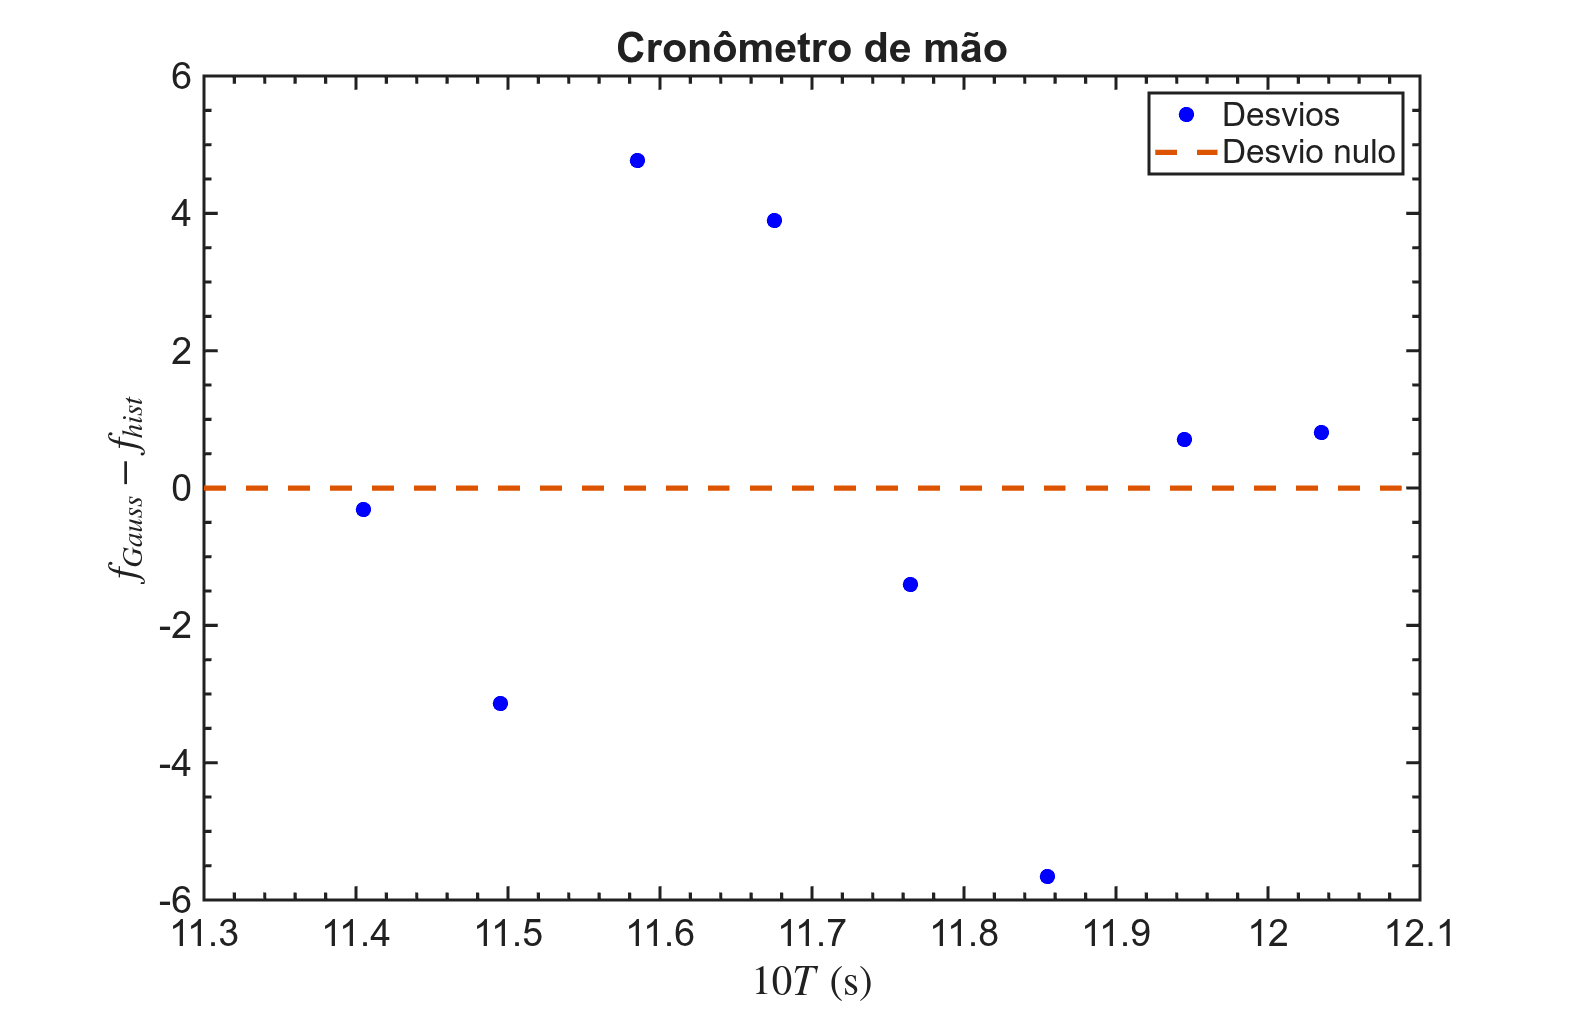
\includegraphics[width=\linewidth]{desvios_cm.png}
	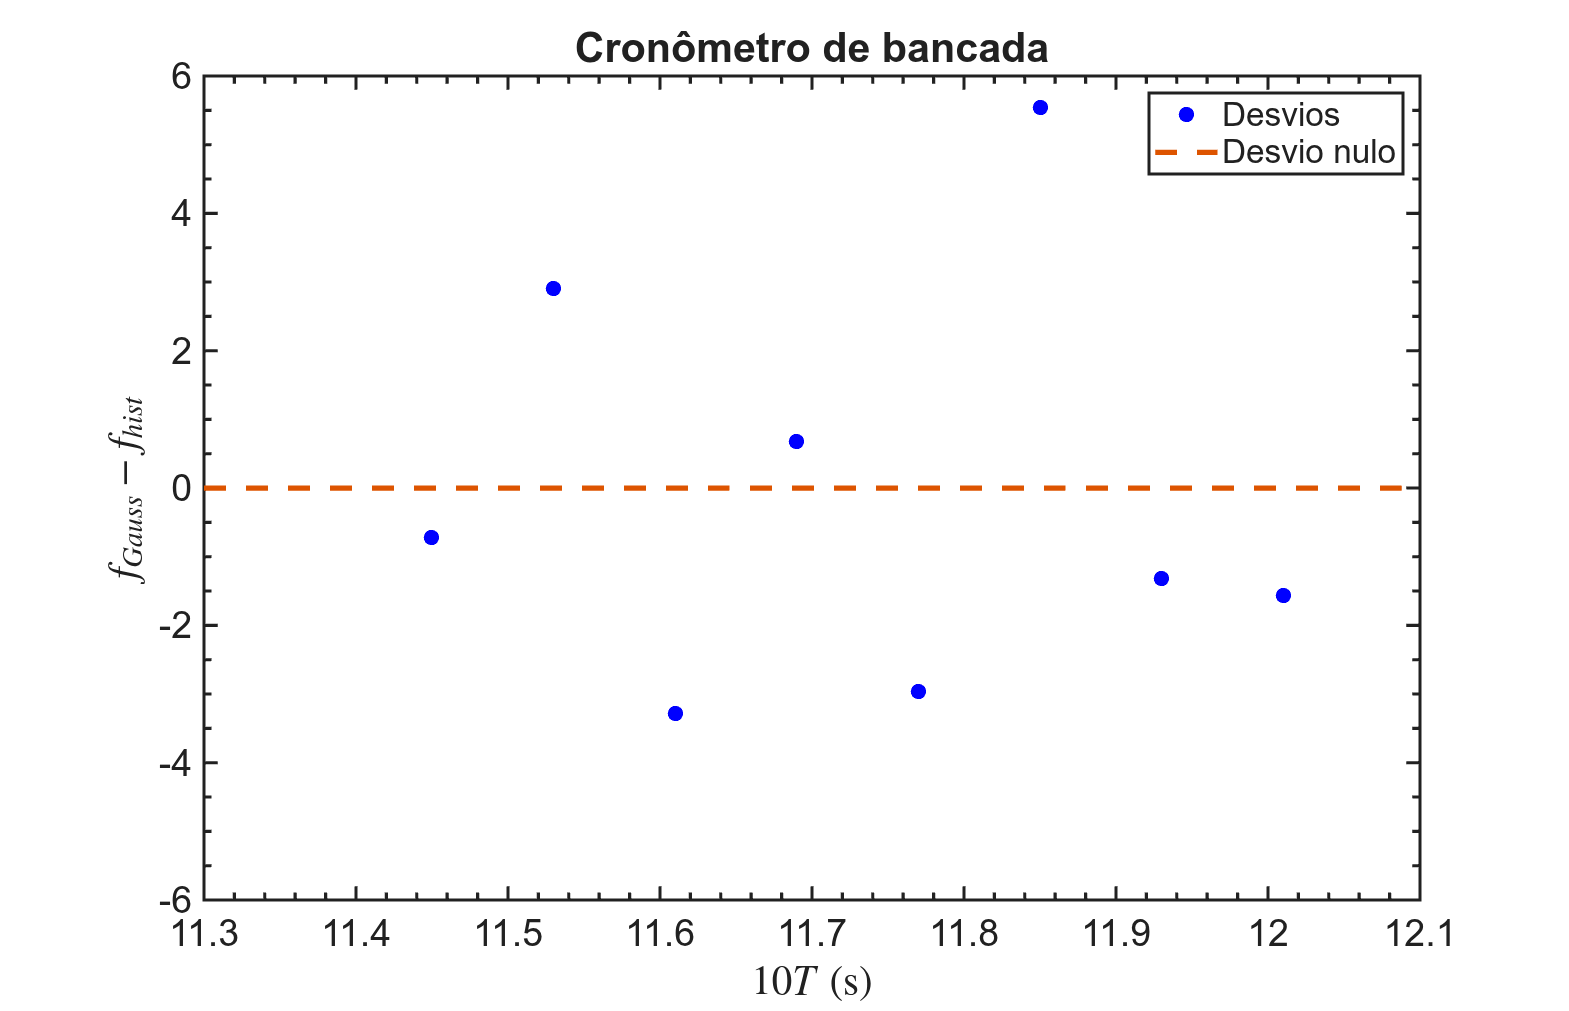
\includegraphics[width=\linewidth]{desvios_cb.png}
	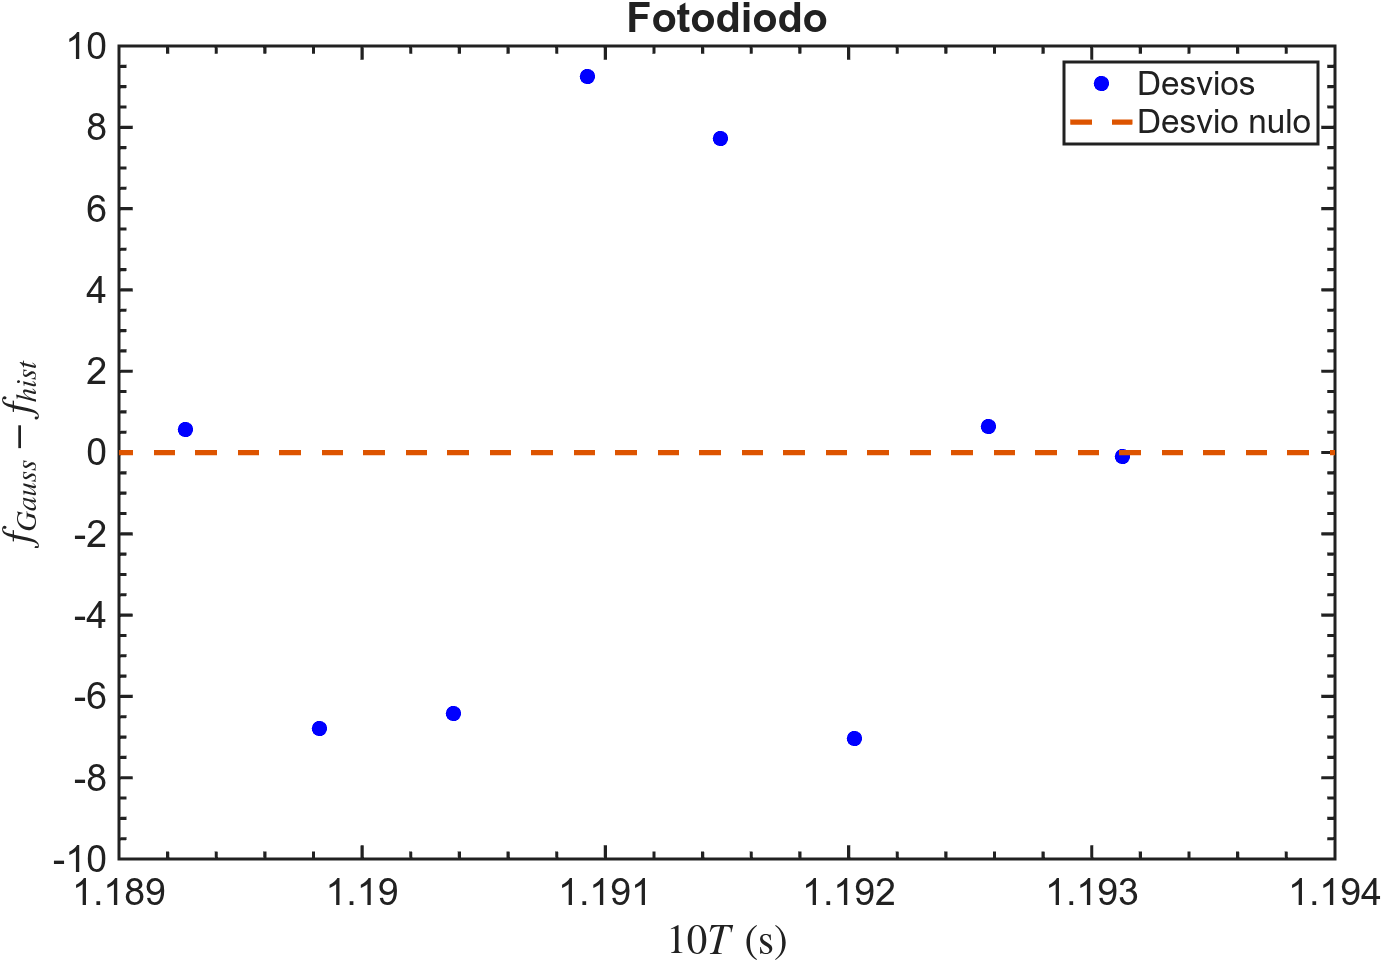
\includegraphics[width=0.9\linewidth]{desvios_fd.png}
	\caption{Desvios clculados para experimento com fotodiodo}
	\label{fig:desvios}
	\end{figure}

    Além da comparação entre distribuições, pode-se comparar os diversos valores de $g$ obtidos experimentalmente e verificar se existe alguma diferença significativa entre os valores obtidos. Para isso, deve-se aplicar um teste de hipótese com $H: g^{(a)}=g^{(b)}$ para quaisquer valores $g^{(a)}$ e $g^{(b)}$ experimentalmente determinados. Para isso, 
    
    \section{Conclusão}
    \bibliography{referencias_relatorio1}
\end{multicols}

\end{document}

